\documentclass[aspectratio=169,11pt]{beamer}

\usepackage[T1]{fontenc}
\usepackage{lmodern}
\usepackage[sfdefault]{FiraSans}
\usepackage{graphicx}
\usepackage{microtype}
\usepackage{tikz}
\usetikzlibrary{arrows.meta,positioning}

\definecolor{EnstaBlue}{HTML}{3645FE}
\definecolor{LisnNavy}{HTML}{202044}
\definecolor{AccentOrange}{HTML}{F47521}
\definecolor{MutedText}{HTML}{667085}
\definecolor{SoftBlue}{HTML}{F4F6FF}
\definecolor{CertifiedGreen}{HTML}{168363}
\definecolor{SoftGreen}{HTML}{ECF8F3}
\definecolor{SoftOrange}{HTML}{FFF3EA}

\setbeamertemplate{navigation symbols}{}
\setbeamercolor{normal text}{fg=LisnNavy,bg=white}
\setbeamercolor{frametitle}{fg=LisnNavy,bg=white}
\setbeamercolor{bibliography entry author}{fg=LisnNavy}
\setbeamercolor{bibliography entry title}{fg=LisnNavy}
\setbeamercolor{bibliography entry location}{fg=MutedText}
\setbeamercolor{bibliography entry note}{fg=MutedText}
\setbeamercolor{demeter takeaway}{fg=LisnNavy,bg=SoftBlue}
\setbeamercolor{certified card}{fg=LisnNavy,bg=SoftGreen}
\setbeamercolor{growth card}{fg=LisnNavy,bg=SoftOrange}
\setbeamercolor{page number in head/foot}{fg=MutedText,bg=white}
\setbeamerfont{normal text}{family=\sffamily}
\setbeamerfont{frametitle}{series=\bfseries,size=\large}
\setbeamertemplate{bibliography item}[text]
\setbeamertemplate{footline}{%
  \hbox to \paperwidth{%
    \hfill
    {\usebeamercolor[fg]{page number in head/foot}%
     \fontsize{5.8}{7}\selectfont
     \insertframenumber\,/\,\inserttotalframenumber}%
    \hspace*{0.42cm}}%
  \vskip0.08cm
}

\graphicspath{{assets/}}

\begin{document}

% Each presentation section lives in its own file so that the deck can grow
% without turning this entry point into a monolithic document.
\begin{frame}[plain]
  \begin{tikzpicture}[remember picture,overlay]
    % A restrained institutional accent at the top of the slide.
    \fill[EnstaBlue]
      (current page.north west)
      rectangle ([yshift=-0.07cm]current page.north east);

    % Institutional logos from the source cover.
    \node[anchor=north west,inner sep=0pt]
      at ([xshift=0.62cm,yshift=-0.44cm]current page.north west)
      {
\includegraphics[width=3.15cm]{ensta.png}};
    \node[anchor=north east,inner sep=0pt]
      at ([xshift=-0.62cm,yshift=-0.30cm]current page.north east)
      {
\includegraphics[width=2.28cm]{lisn.png}};

    % Programme and academic context.
    \node[anchor=north,align=center,text=LisnNavy]
      at ([yshift=-0.39cm]current page.north)
      {\fontsize{8.7}{10.4}\selectfont\bfseries RESEARCH PROJECT (PRe)};
    \node[anchor=north,align=center,text=MutedText]
      at ([yshift=-0.82cm]current page.north)
      {\fontsize{6.7}{8.2}\selectfont\bfseries ACADEMIC YEAR 2026--2027};
    \node[anchor=north,align=center,text width=13.3cm,text=LisnNavy]
      at ([yshift=-1.20cm]current page.north)
      {\fontsize{7.1}{8.8}\selectfont
       \textbf{Specialization:} Information and Communication Sciences and
       Technologies (STIC)};

    \draw[MutedText!28,line width=0.35pt]
      ([xshift=1.15cm,yshift=-1.72cm]current page.north west) --
      ([xshift=-1.15cm,yshift=-1.72cm]current page.north east);

    % Project title and subtitle.
    \node[anchor=north,align=center,text width=13.7cm,text=LisnNavy]
      at ([yshift=-2.06cm]current page.north)
      {\fontsize{17.2}{20.2}\selectfont\bfseries
       \textcolor{EnstaBlue}{CAGE-NAS:} Certified Adaptive Growth\\[-0.01cm]
       and Expansion\\[-0.01cm]
       for Neural Architecture Search};
    \node[anchor=north,align=center,text width=14.0cm,text=MutedText]
      at ([yshift=-4.08cm]current page.north)
      {\fontsize{8.7}{10.5}\selectfont
       Toward Resource-Aware Deep Learning through Adaptive Capacity Allocation};

    \fill[AccentOrange]
      ([xshift=-0.40cm,yshift=-4.63cm]current page.north) rectangle
      ([xshift=0.40cm,yshift=-4.57cm]current page.north);

    % Project details: three balanced cards keep the dense cover information
    % readable on a landscape presentation slide.
    \node[anchor=north,rounded corners=2pt,fill=SoftBlue,
          minimum width=4.45cm,minimum height=1.64cm,inner sep=0.18cm,
          align=left,text width=3.92cm]
      at ([xshift=-5.05cm,yshift=-4.89cm]current page.north)
      {\fontsize{6.5}{8}\selectfont\bfseries\color{MutedText}AUTHOR\\[0.07cm]
       \fontsize{9.2}{11}\selectfont\color{LisnNavy}Santiago Florido Gomez\\[0.16cm]
       \fontsize{6.5}{8}\selectfont\bfseries\color{MutedText}CLASS\enspace
       \fontsize{8.2}{10}\selectfont\color{LisnNavy}2027};

    \node[anchor=north,rounded corners=2pt,fill=SoftBlue,
          minimum width=4.45cm,minimum height=1.64cm,inner sep=0.18cm,
          align=left,text width=3.92cm]
      at ([yshift=-4.89cm]current page.north)
      {\fontsize{6.5}{8}\selectfont\bfseries\color{MutedText}
       ENSTA PARIS SUPERVISOR\\[0.12cm]
       \fontsize{9.2}{11}\selectfont\color{EnstaBlue}Zhi Yan};

    \node[anchor=north,rounded corners=2pt,fill=SoftBlue,
          minimum width=4.45cm,minimum height=1.64cm,inner sep=0.18cm,
          align=left,text width=3.92cm]
      at ([xshift=5.05cm,yshift=-4.89cm]current page.north)
      {\fontsize{6.5}{8}\selectfont\bfseries\color{MutedText}
       HOST ORGANIZATION SUPERVISOR\\[0.12cm]
       \fontsize{9.2}{11}\selectfont\color{EnstaBlue}St\'ephane Rivaud};

    % Internship period and host organization.
    \node[anchor=north,align=center,text width=14.0cm,text=LisnNavy]
      at ([yshift=-6.89cm]current page.north)
      {\fontsize{8.2}{10}\selectfont
       \textbf{Internship carried out from May 18, 2026 to August 14, 2026}};
    \node[anchor=north,align=center,text width=14.0cm,text=MutedText]
      at ([yshift=-7.39cm]current page.north)
      {\fontsize{7.8}{9.7}\selectfont
       \textbf{Host Organization:} Interdisciplinary Laboratory of Digital
       Sciences (LISN)};

    % Bottom rule visually closes the cover without adding footer chrome.
    \draw[EnstaBlue,line width=0.75pt]
      ([xshift=0.62cm,yshift=0.40cm]current page.south west) --
      ([xshift=-0.62cm,yshift=0.40cm]current page.south east);
  \end{tikzpicture}
\end{frame}

\section{What DEMETER Reveals about Train-and-Grow Optimization}

\begin{frame}[t]{What DEMETER Reveals about Train-and-Grow Optimization}
  \vspace{-0.08cm}
  \begin{columns}[T,onlytextwidth]
    \begin{column}{0.37\textwidth}
      {\fontsize{7.4}{9}\selectfont\bfseries\color{EnstaBlue}
       WHY ALIGNMENT BREAKS}

      \vspace{0.15cm}
      \begin{itemize}
        \setlength\itemsep{0.12cm}
        \fontsize{8.2}{10.2}\selectfont

        \item \textbf{Growth is function-directed.}
        New capacity is selected to align a local functional-gradient
        projection.

        \item \textbf{Training is parameter-directed.}
        SGD moves in parameter space; its Jacobian-induced effect generally
        follows a different function-space direction.

        \item \textbf{The directions can conflict.}
        Interleaving them can redirect progress; overtraining between growth
        events may favor local minima \textcolor{MutedText}{(Douka et al., 2025)}.
      \end{itemize}

      \vspace{0.08cm}
      \begin{beamercolorbox}[rounded=true,sep=0.17cm,wd=\linewidth]{demeter takeaway}
        \fontsize{7.6}{9.5}\selectfont
        \textbf{Key observation.} Alignment is episodic, not sustained.
        Cosine peaks mark growth epochs; between them, parametric training
        remains weakly aligned.
      \end{beamercolorbox}
    \end{column}

    \begin{column}{0.60\textwidth}
      \centering
      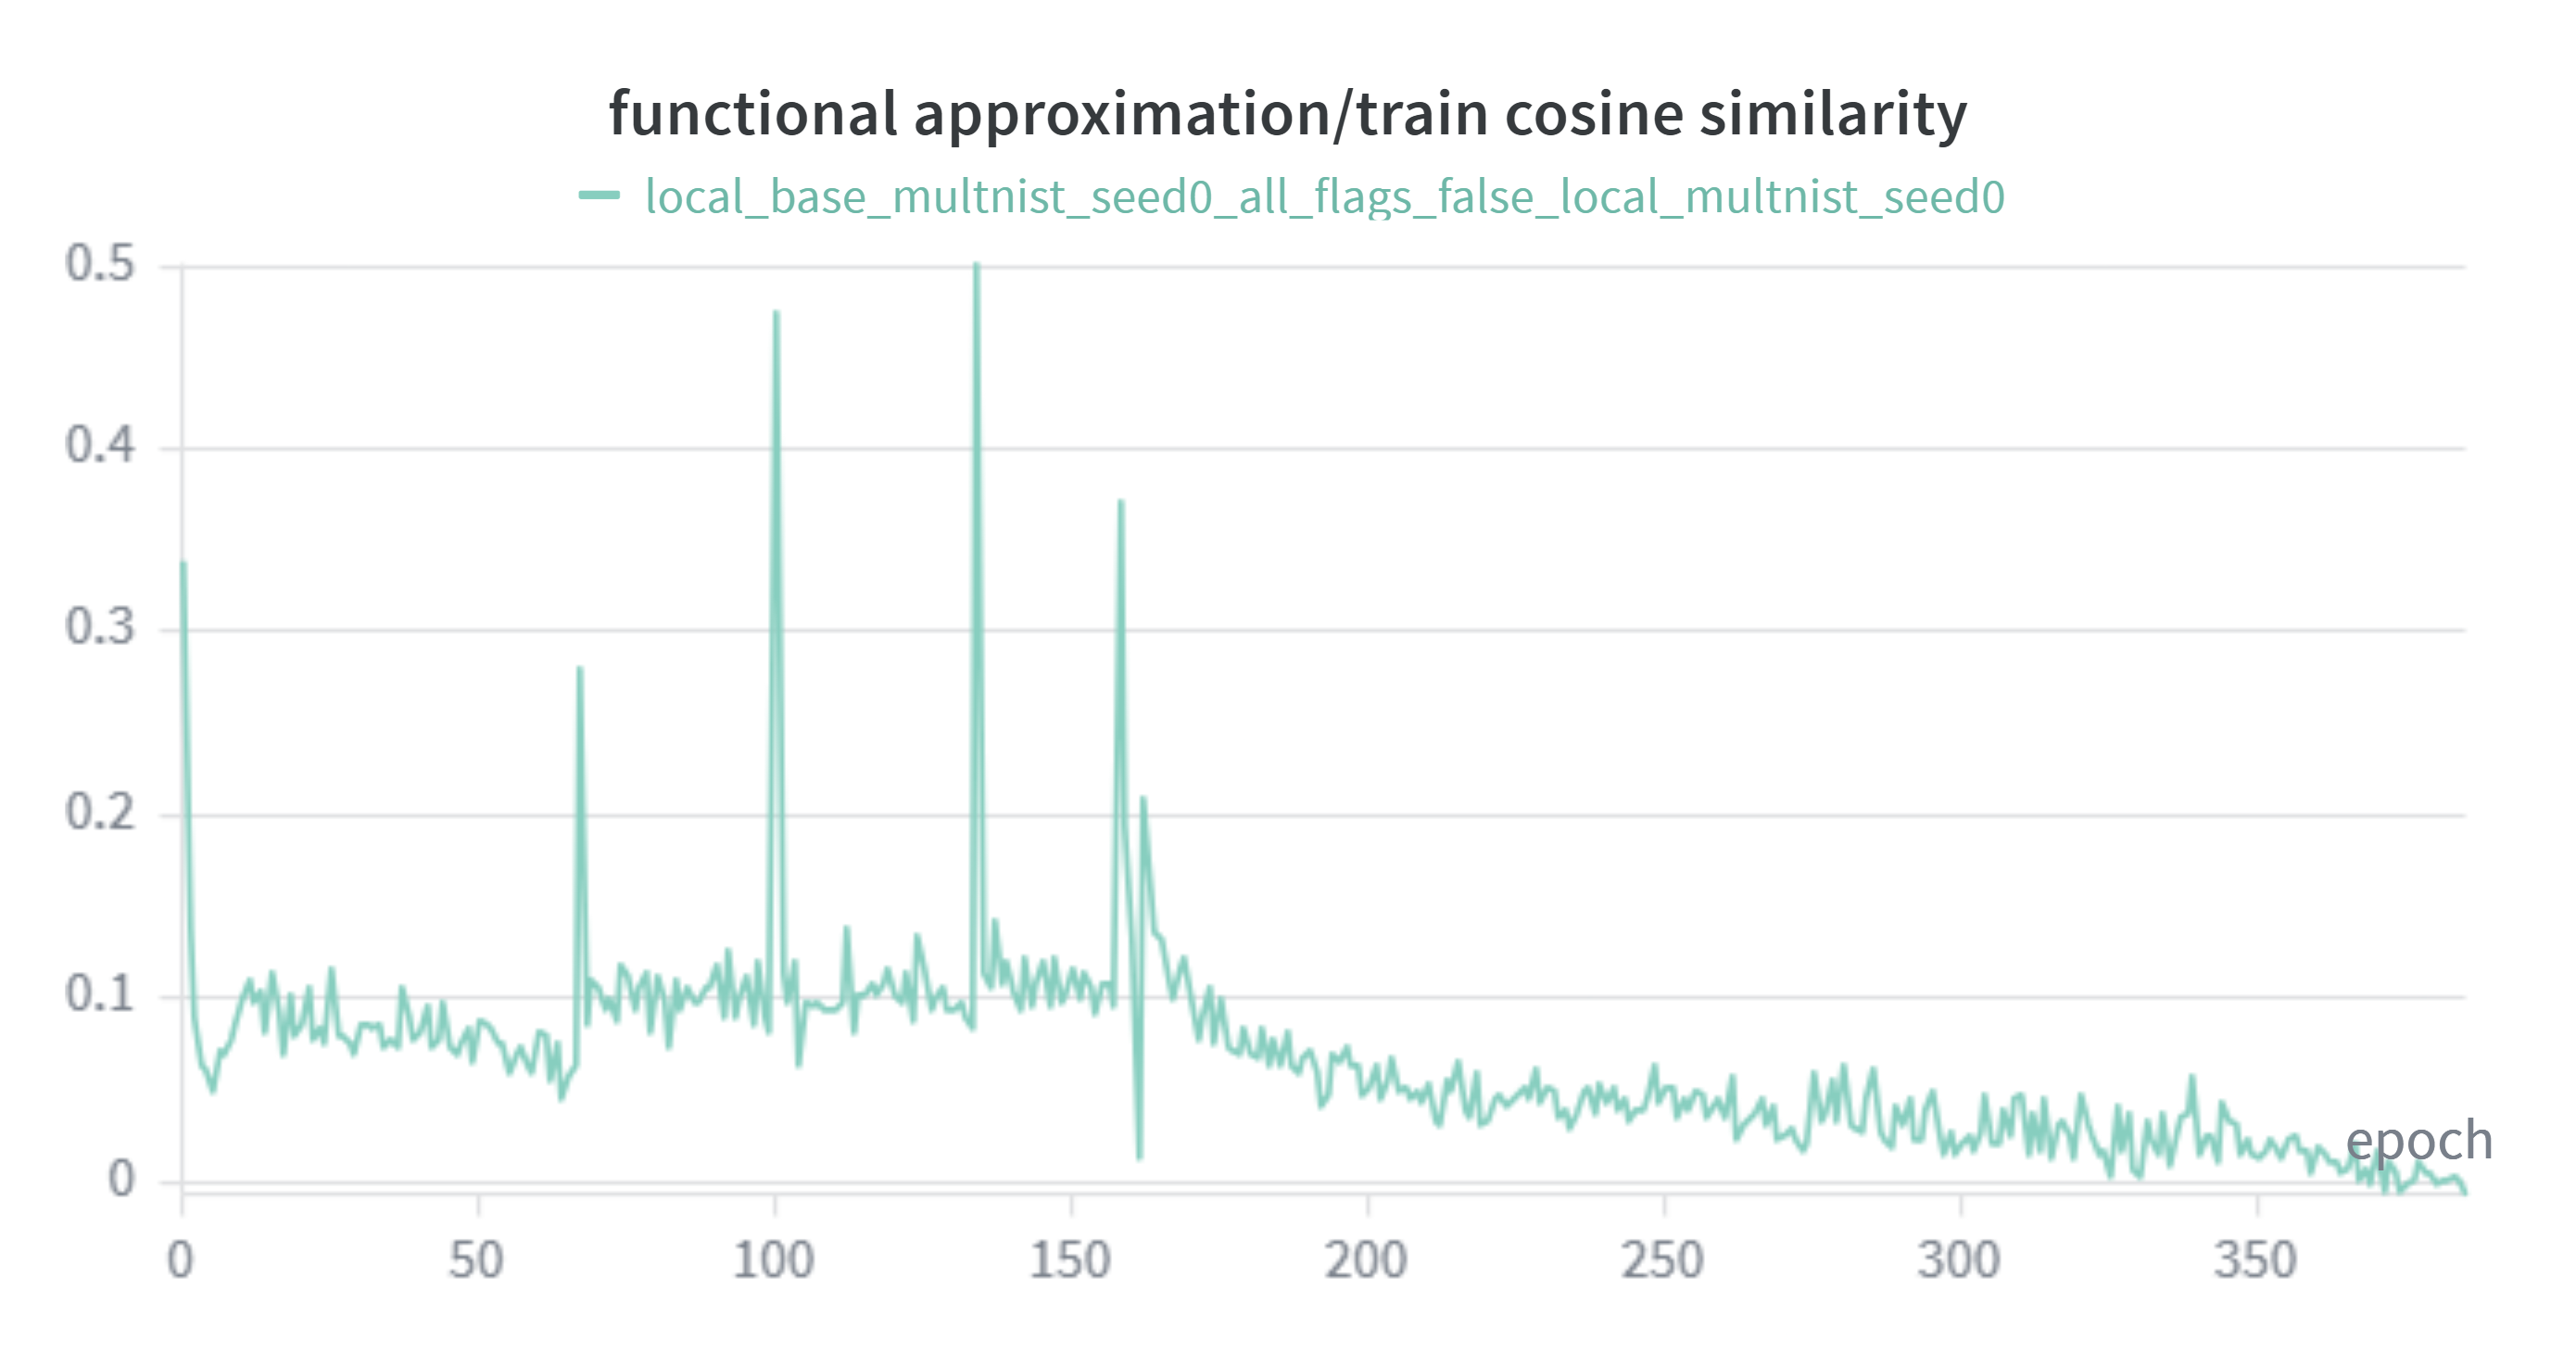
\includegraphics[width=\linewidth]{demeter_cosine_similarity.png}

      \vspace{0.05cm}
      \parbox{0.96\linewidth}{%
        \centering
        \fontsize{6.5}{8.0}\selectfont\color{MutedText}
        \textbf{Figure 4:} MultiNIST cosine similarity between the functional
        gradient and the zeroth-order contribution during DEMETER training and
        growth.%
      }
    \end{column}
  \end{columns}
\end{frame}

\section{Adaptive Representations for Function-Space Optimization}

\begin{frame}[t]{Adaptive Representations for Function-Space Optimization}
  \vspace{-0.10cm}
  \begin{columns}[T,onlytextwidth]
    \begin{column}{0.585\textwidth}
      {\color{EnstaBlue}\bfseries\scriptsize FROM THE IDEAL STEP TO A REALIZABLE UPDATE}
      \vspace{0.03cm}

      \begin{beamercolorbox}[rounded=true,sep=0.10cm,wd=\linewidth]{demeter takeaway}
        \centering
        \fontsize{7.3}{8.6}\selectfont
        \(\displaystyle
          \begin{gathered}
            \min_{f\in\mathcal H}\mathcal L(f),
            \qquad f_{t+1}=f_t-\eta\nabla\mathcal L(f_t),\\[3pt]
            \text{finite approximation:}\quad
            f_{t+1}=f_t-\eta g_t,\quad g_t\in\mathcal B.
          \end{gathered}
        \)
      \end{beamercolorbox}

      \vspace{0.10cm}
      {\color{EnstaBlue}\bfseries\scriptsize APPROXIMATION CERTIFICATE}
      \vspace{0.03cm}

      \begin{beamercolorbox}[rounded=true,sep=0.10cm,wd=\linewidth]{demeter takeaway}
        \centering
        \fontsize{7.0}{8.3}\selectfont
        \(\displaystyle
          \begin{gathered}
            \varepsilon_t
            =\frac{\lVert g_t-\nabla\mathcal L(f_t)\rVert_{\mathcal B}}
                   {\lVert g_t\rVert_{\mathcal B}},\\[4pt]
            \mathcal L(f_{t+1})\leq \mathcal L(f_t)
            -\eta q_t\lVert\nabla\mathcal L(f_t)\rVert_{\mathcal B}^{2},\\[4pt]
            q_t:=\alpha-\frac{K\eta}{2}
            -\left(\beta+\frac{3K\eta}{2}\right)
             \frac{\varepsilon_t}{1-\varepsilon_t}.
          \end{gathered}
        \)
      \end{beamercolorbox}

      \vspace{0.09cm}
      {\fontsize{7.35}{8.8}\selectfont
      With $K$-smoothness, verifiable descent, and compatibility, $q_t>0$
      certifies loss decrease despite the approximation.}
    \end{column}

    \begin{column}{0.385\textwidth}
      {\color{EnstaBlue}\bfseries\scriptsize WHY ADAPT THE REPRESENTATION?}
      \vspace{0.03cm}

      {\fontsize{7.35}{8.8}\selectfont
      \begin{itemize}
        \setlength{\itemsep}{0.08cm}
        \item $\mathcal H$ can be infinite-dimensional, but updates are
              finite; growth enriches the representation and reduces
              $\varepsilon_t$.
        \item Once $q_t>0$, training and growth follow the same certified
              function-space descent.
      \end{itemize}}

      \vspace{0.03cm}
      {\color{EnstaBlue}\bfseries\scriptsize SUFFICIENT CONDITIONS}
      \vspace{0.03cm}

      \begin{beamercolorbox}[rounded=true,sep=0.10cm,wd=\linewidth]{demeter takeaway}
        \centering
        \fontsize{6.6}{8.0}\selectfont
        \(\displaystyle
          \begin{gathered}
            \eta<\frac{2\,[\alpha-(\alpha+\beta)\varepsilon]}
                         {K(2\varepsilon+1)},\qquad \varepsilon_t\leq\varepsilon,\\[4pt]
            \mathcal L(f)-\mathcal L^*
            \leq \frac{1}{2\mu}
            \lVert D\mathcal L(f;\cdot)\rVert_{\mathcal B^*}^{2}.
          \end{gathered}
        \)
      \end{beamercolorbox}

      \vspace{0.09cm}
      \begin{beamercolorbox}[rounded=true,sep=0.10cm,wd=\linewidth]{demeter takeaway}
        {\fontsize{7.15}{8.5}\selectfont\bfseries\color{LisnNavy}
        With PL (or convex MSE), certified descent converges globally;
        approximation quality determines when the model must grow.}
      \end{beamercolorbox}

      \vspace{0.04cm}
      {\color{MutedText}\fontsize{6.2}{7.3}\selectfont
      Framework summarized from Csillag et al. (2026).}
    \end{column}
  \end{columns}
\end{frame}

\section{CAGE-NAS}

\begin{frame}[t]{CAGE-NAS: Certified Train-and-Grow Search}
  \vspace{-0.08cm}
  {\fontsize{8.0}{9.5}\selectfont
  Starting from a deliberately small network, CAGE-NAS expands capacity only
  when the current architecture cannot realize a certified approximation of
  the functional gradient.}

  \vspace{0.12cm}
  \begin{center}
    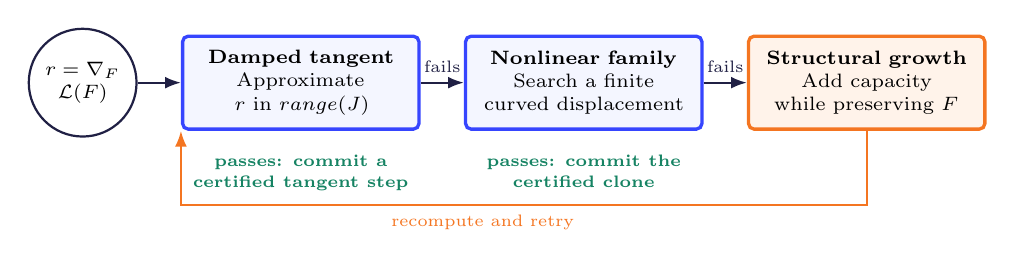
\begin{tikzpicture}[
      node distance=0.50cm,
      stage/.style={draw=EnstaBlue, rounded corners=2pt, very thick,
        fill=SoftBlue, align=center, inner sep=5pt,
        text width=2.65cm, minimum height=1.18cm,
        font=\fontsize{7.1}{8.4}\selectfont},
      growthstage/.style={draw=AccentOrange, rounded corners=2pt, very thick,
        fill=SoftOrange, align=center, inner sep=5pt,
        text width=2.65cm, minimum height=1.18cm,
        font=\fontsize{7.1}{8.4}\selectfont},
      signal/.style={draw=LisnNavy, circle, thick, fill=white,
        align=center, inner sep=3pt, minimum size=1.08cm,
        font=\fontsize{7.0}{8.2}\selectfont},
      flow/.style={-{Latex[length=2mm]}, thick, color=LisnNavy}
    ]
      \node[signal] (grad) {$r=\nabla_F$\\$\mathcal L(F)$};
      \node[stage, right=0.55cm of grad] (tangent)
        {\textbf{Damped tangent}\\Approximate $r$ in $\operatorname{range}(J)$};
      \node[stage, right=0.55cm of tangent] (nonlinear)
        {\textbf{Nonlinear family}\\Search a finite curved displacement};
      \node[growthstage, right=0.55cm of nonlinear] (growth)
        {\textbf{Structural growth}\\Add capacity while preserving $F$};

      \draw[flow] (grad) -- (tangent);
      \draw[flow] (tangent) -- node[above, font=\fontsize{6.2}{7.2}\selectfont]
        {fails} (nonlinear);
      \draw[flow] (nonlinear) -- node[above, font=\fontsize{6.2}{7.2}\selectfont]
        {fails} (growth);

      \node[below=0.18cm of tangent, text=CertifiedGreen,
        font=\fontsize{6.5}{7.7}\selectfont\bfseries, align=center]
        {passes: commit a\\certified tangent step};
      \node[below=0.18cm of nonlinear, text=CertifiedGreen,
        font=\fontsize{6.5}{7.7}\selectfont\bfseries, align=center]
        {passes: commit the\\certified clone};

      \draw[-{Latex[length=2mm]}, thick, color=AccentOrange]
        (growth.south) -- ++(0,-0.94cm) -| node[pos=0.28,below,
        font=\fontsize{6.2}{7.2}\selectfont] {recompute and retry}
        (tangent.south west);
    \end{tikzpicture}
  \end{center}

  \vspace{-0.06cm}
  \begin{columns}[T,onlytextwidth]
    \begin{column}{0.49\textwidth}
      {\color{EnstaBlue}\bfseries\scriptsize ONE CERTIFICATE FOR BOTH FAMILIES}
      \vspace{0.03cm}

      \begin{beamercolorbox}[rounded=true,sep=0.11cm,wd=\linewidth]{certified card}
        \centering
        \fontsize{7.0}{8.3}\selectfont
        \(\displaystyle
          \operatorname{RelErr}(g,r)
          =\frac{\lVert g-r\rVert_2}{\lVert g\rVert_2}
          <\frac12
        \)
      \end{beamercolorbox}
    \end{column}

    \begin{column}{0.49\textwidth}
      {\color{EnstaBlue}\bfseries\scriptsize CONSTRUCTIVE ARCHITECTURE SEARCH}
      \vspace{0.03cm}

      \begin{beamercolorbox}[rounded=true,sep=0.11cm,wd=\linewidth]{growth card}
        \centering
        \fontsize{6.9}{8.2}\selectfont
        \(\displaystyle
          A_0\prec A_1\prec\cdots,
          \qquad F_{A^+,\theta^+}=F_{A,\theta}
        \)
      \end{beamercolorbox}
    \end{column}
  \end{columns}

  \vspace{0.10cm}
  \begin{beamercolorbox}[rounded=true,sep=0.10cm,wd=\linewidth]{demeter takeaway}
    {\fontsize{7.3}{8.7}\selectfont\bfseries
    Certification answers \emph{when} growth is necessary; counterfactual
    candidate certificates determine \emph{where} capacity should be added.}
  \end{beamercolorbox}
\end{frame}

\subsection{Damped Tangent Family}

\begin{frame}[t]{The Damped Tangent Family}
  \vspace{-0.08cm}
  {\fontsize{7.6}{9.0}\selectfont
  The first candidate approximates $r$ in the network tangent space while
  penalizing unsafe parameter motion.}

  \vspace{0.11cm}
  \begin{columns}[T,onlytextwidth]
    \begin{column}{0.555\textwidth}
      {\color{EnstaBlue}\bfseries\scriptsize REGULARIZED TANGENT PROJECTION}
      \vspace{0.04cm}

      \begin{beamercolorbox}[rounded=true,sep=0.12cm,wd=\linewidth]{demeter takeaway}
        \centering
        \fontsize{7.0}{8.3}\selectfont
        \(\displaystyle
          \begin{gathered}
            u_\lambda=\operatorname*{arg\,min}_{u\in\mathbb R^{p_A}}
            \left\{\lVert Ju-r\rVert_2^2+\lambda\lVert u\rVert_2^2\right\},\\[5pt]
            g_\lambda=Ju_\lambda\in\operatorname{range}(J).
          \end{gathered}
        \)
      \end{beamercolorbox}

      \vspace{0.11cm}
      {\color{EnstaBlue}\bfseries\scriptsize MODE-BY-MODE SOLUTION}
      \vspace{0.04cm}

      \begin{beamercolorbox}[rounded=true,sep=0.12cm,wd=\linewidth]{demeter takeaway}
        \centering
        \fontsize{6.8}{8.1}\selectfont
        \(\displaystyle
          \begin{gathered}
            J=U\Sigma V^\top,\qquad a=U^\top r,\\[4pt]
            u_\lambda
            =V\operatorname{diag}\!\left(
              \frac{\sigma_i}{\sigma_i^2+\lambda}
            \right)a,\\[4pt]
            g_\lambda
            =U\operatorname{diag}\!\left(
              \frac{\sigma_i^2}{\sigma_i^2+\lambda}
            \right)a.
          \end{gathered}
        \)
      \end{beamercolorbox}

      \vspace{0.08cm}
      {\fontsize{6.9}{8.2}\selectfont
      Damping limits $\lVert u\rVert_2$, controlling nonlinear realization error.}
    \end{column}

    \begin{column}{0.415\textwidth}
      {\color{EnstaBlue}\bfseries\scriptsize SPECTRAL FILTER}
      \vspace{0.04cm}

      \begin{beamercolorbox}[rounded=true,sep=0.10cm,wd=\linewidth]{certified card}
        \centering
        \fontsize{7.0}{8.3}\selectfont
        \(\displaystyle
          h_i(\lambda)=\frac{\sigma_i^2}{\sigma_i^2+\lambda}\in[0,1]
        \)
      \end{beamercolorbox}

      \vspace{0.04cm}
      {\fontsize{7.2}{8.6}\selectfont
      \begin{itemize}
        \setlength{\itemsep}{0.07cm}
        \item $\sigma_i^2\gg\lambda$: transmit the reachable component.
        \item $\sigma_i^2\ll\lambda$: suppress an ill-conditioned mode.
        \item $\sigma_i=0$: the direction is structurally unreachable.
      \end{itemize}}

      \vspace{0.03cm}
      {\color{EnstaBlue}\bfseries\scriptsize CERTIFICATE AND SCALE}
      \vspace{0.04cm}

      \begin{beamercolorbox}[rounded=true,sep=0.10cm,wd=\linewidth]{certified card}
        \centering
        \fontsize{6.8}{8.1}\selectfont
        \(\displaystyle
          \begin{gathered}
            \varepsilon_\lambda
            =\frac{\lVert g_\lambda-r\rVert_2}{\lVert g_\lambda\rVert_2}
            <\frac12,\\[4pt]
            \lambda=\rho\,\sigma_{\max}^2,\qquad
            \rho\in[10^{-16},10^2].
          \end{gathered}
        \)
      \end{beamercolorbox}

      \vspace{0.08cm}
      \begin{beamercolorbox}[rounded=true,sep=0.09cm,wd=\linewidth]{growth card}
        \centering
        {\fontsize{6.7}{8.0}\selectfont
        \textbf{Undamped limit:}\quad
        $\varepsilon<\tfrac12\Rightarrow
        \lVert r_{\parallel}\rVert_2^2>0.8\lVert r\rVert_2^2$.}
      \end{beamercolorbox}
    \end{column}
  \end{columns}
\end{frame}

\subsection{Nonlinear Parametric Displacement Family}

\begin{frame}[t]{The Nonlinear Parametric Displacement Family}
  \vspace{-0.18cm}
  {\fontsize{7.5}{8.9}\selectfont
  If tangent projection fails, a clone searches a finite curved trajectory
  within the same architecture.}

  \vspace{0.10cm}
  \begin{columns}[T,onlytextwidth]
    \begin{column}{0.525\textwidth}
      {\color{EnstaBlue}\bfseries\scriptsize ESCAPING THE INITIAL TANGENT PLANE}
      \vspace{0.04cm}

      \begin{beamercolorbox}[rounded=true,sep=0.11cm,wd=\linewidth]{demeter takeaway}
        \centering
        \fontsize{6.9}{8.2}\selectfont
        \(\displaystyle
          F(\theta(T))-F(\theta(0))
          =\int_0^T J_{A,\theta(t)}\dot\theta(t)\,\mathrm dt
        \)
      \end{beamercolorbox}

      \vspace{0.10cm}
      {\color{EnstaBlue}\bfseries\scriptsize REFLECTED TRAINING TARGET}
      \vspace{0.04cm}

      \begin{beamercolorbox}[rounded=true,sep=0.11cm,wd=\linewidth]{demeter takeaway}
        \centering
        \fontsize{7.0}{8.3}\selectfont
        \(\displaystyle
          \begin{gathered}
            r=2(F-Y),\qquad \eta_f=1,\\[4pt]
            F_{\mathrm{target}}=F-r=2Y-F.
          \end{gathered}
        \)
      \end{beamercolorbox}

      \vspace{0.10cm}
      {\color{EnstaBlue}\bfseries\scriptsize REALIZED NONLINEAR DIRECTION}
      \vspace{0.04cm}

      \begin{beamercolorbox}[rounded=true,sep=0.11cm,wd=\linewidth]{growth card}
        \centering
        \fontsize{7.0}{8.3}\selectfont
        \(\displaystyle
          \Delta=F(\theta)-F(\widetilde\theta)
        \)
      \end{beamercolorbox}

      \vspace{0.08cm}
      {\fontsize{6.9}{8.2}\selectfont
      The reflected target lets $\Delta$ exploit higher-order effects beyond
      the initial tangent plane.}
    \end{column}

    \begin{column}{0.445\textwidth}
      {\color{EnstaBlue}\bfseries\scriptsize SCALE-FREE ANGULAR CERTIFICATE}
      \vspace{0.04cm}

      \begin{beamercolorbox}[rounded=true,sep=0.11cm,wd=\linewidth]{certified card}
        \centering
        \fontsize{6.8}{8.1}\selectfont
        \(\displaystyle
          \begin{gathered}
            \chi=\frac{\langle\Delta,r\rangle}
            {\lVert\Delta\rVert_2\lVert r\rVert_2},\\[5pt]
            \varepsilon_{\mathrm{NL}}^\star
            =\sqrt{1-\max\{\chi,0\}^2}.
          \end{gathered}
        \)
      \end{beamercolorbox}

      \vspace{0.10cm}
      {\color{EnstaBlue}\bfseries\scriptsize ADMISSIBILITY}
      \vspace{0.04cm}

      \begin{beamercolorbox}[rounded=true,sep=0.11cm,wd=\linewidth]{certified card}
        \centering
        \fontsize{6.9}{8.2}\selectfont
        \(\displaystyle
          \chi>0,\quad \varepsilon_{\mathrm{NL}}^\star<\frac12
          \quad\Longleftrightarrow\quad
          \chi>\frac{\sqrt3}{2}
        \)
      \end{beamercolorbox}

      \vspace{0.10cm}
      {\color{EnstaBlue}\bfseries\scriptsize RAY-OPTIMAL SCALING}
      \vspace{0.04cm}

      \begin{beamercolorbox}[rounded=true,sep=0.11cm,wd=\linewidth]{growth card}
        \centering
        \fontsize{6.9}{8.2}\selectfont
        \(\displaystyle
          a^\star=\frac{\lVert r\rVert_2^2}{\langle\Delta,r\rangle},
          \qquad g_{\mathrm{NL}}=a^\star\Delta\approx r
        \)
      \end{beamercolorbox}

      \vspace{0.09cm}
      {\fontsize{6.9}{8.2}\selectfont
      $\chi$ certifies orientation; $a^\star$ corrects magnitude.}
    \end{column}
  \end{columns}

  \begin{beamercolorbox}[rounded=true,sep=0.06cm,wd=\linewidth]{demeter takeaway}
    \centering
    {\fontsize{6.9}{8.2}\selectfont\bfseries
    Pass $\rightarrow$ commit the nonlinear clone.\qquad
    Fail $\rightarrow$ trigger function-preserving growth.}
  \end{beamercolorbox}
\end{frame}

\section{References}

\begin{frame}[allowframebreaks=0.88]{References}
  \fontsize{7.2}{8.8}\selectfont
  \begin{thebibliography}{99}

  \bibitem[Poyser \& Breckon(2024)]{poyser2024nas}
  Poyser, M.\ \& Breckon, T.~P.\ (2024).
  \textit{Neural Architecture Search: A Contemporary Literature Review for
  Computer Vision Applications}.
  Pattern Recognition, vol.\ 147, p.\ 110052.
  \url{https://doi.org/10.1016/j.patcog.2023.110052}.

  \bibitem[Goebel et~al.(2012)]{goebel2012hybrid}
  Goebel, R., Sanfelice, R.G.\ \& Teel, A.R.\ (2012).
  \textit{Hybrid Dynamical Systems: Modeling, Stability, and Robustness}.
  Princeton, NJ: Princeton University Press.

  \bibitem[Desislavov et~al.(2023)]{desislavov2023compute}
  Desislavov, R., Mart\'inez-Plumed, F.\ \& Hern\'andez-Orallo, J.\ (2023).
  \textit{Compute and Energy Consumption Trends in Deep Learning Inference}.
  Sustainable Computing: Informatics and Systems, vol.\ 38, p.\ 100857.
  \url{https://doi.org/10.1016/j.suscom.2023.100857}.

  \bibitem[Hornik et~al.(1989)]{hornik1989multilayer}
  Hornik, K., Stinchcombe, M.\ \& White, H.\ (1989).
  \textit{Multilayer Feedforward Networks Are Universal Approximators}.
  Neural Networks, vol.\ 2, no.\ 5, pp.\ 359--366.
  \url{https://doi.org/10.1016/0893-6080(89)90020-8}.

  \bibitem[Cybenko(1989)]{cybenko1989approximation}
  Cybenko, G.\ (1989).
  \textit{Approximation by Superpositions of a Sigmoidal Function}.
  Mathematics of Control, Signals and Systems, vol.\ 2, no.\ 4, pp.\ 303--314.
  \url{https://doi.org/10.1007/BF02551274}.

  \bibitem[Bahri et~al.(2024)]{bahri2024explaining}
  Bahri, Y., Dyer, E., Kaplan, J., Lee, J.\ \& Sharma, U.\ (2024).
  \textit{Explaining Neural Scaling Laws}.
  Proceedings of the National Academy of Sciences, vol.\ 121, no.\ 27,
  p.\ e2311878121.
  \url{https://doi.org/10.1073/pnas.2311878121}.

  \framebreak

  \bibitem[Kumar et~al.(2024)]{kumar2024cegi}
  Kumar, A., Pathak, K., Kavuru, R.\ \& Srinivasan, P.\ (2024).
  \textit{CEGI: Measuring the Trade-off Between Efficiency and Carbon
  Emissions for SLMs and VLMs}.
  arXiv preprint arXiv:2412.02602 [cs.CL].
  \url{https://doi.org/10.48550/arXiv.2412.02602}.

  \bibitem[Hassani et~al.(2021)]{hassani2021compact}
  Hassani, A., Walton, S., Shah, N., Abuduweili, A., Li, J.\ \& Shi, H.\ (2021).
  \textit{Escaping the Big Data Paradigm with Compact Transformers}.
  arXiv preprint arXiv:2104.05704 [cs.CV].
  \url{https://doi.org/10.48550/arXiv.2104.05704}.

  \bibitem[Verbockhaven et~al.(2024)]{verbockhaven2024growing}
  Verbockhaven, M., Rudkiewicz, T., Chevallier, S.\ \& Charpiat, G.\ (2024).
  \textit{Growing Tiny Networks: Spotting Expressivity Bottlenecks and Fixing
  Them Optimally}.
  Transactions on Machine Learning Research.
  \url{https://openreview.net/forum?id=hbtG6s6e7r}.

  \bibitem[Douka et~al.(2025)]{douka2025growth}
  Douka, S., Verbockhaven, M., Rudkiewicz, T., Rivaud, S., Landes, F.P.,
  Chevallier, S.\ \& Charpiat, G.\ (2025).
  \textit{Growth Strategies for Arbitrary DAG Neural Architectures}.
  Proceedings of the 33rd European Symposium on Artificial Neural Networks,
  Computational Intelligence and Machine Learning (ESANN), pp.\ 443--448.
  Bruges, Belgium: i6doc.com.
  \url{https://doi.org/10.14428/esann/2025.ES2025-112}.

  \bibitem[Csillag et~al.(2026)]{csillag2026functional}
  Csillag, D., Schuller, R., Dall'Antonia, P., Guibas, L., Velho, L.\ \&
  Novello, T.\ (2026).
  \textit{Functional Gradient Descent with Adaptive Representations}.
  arXiv preprint arXiv:2606.16926v1 [math.OC].
  \url{https://doi.org/10.48550/arXiv.2606.16926}.

  \bibitem[Rudkiewicz(2024)]{rudkiewicz2024fogro}
  Rudkiewicz, Th\'eo (2024).
  \textit{FOGro: First-Order Neural Network Growth}.
  Master's thesis, \'Ecole normale sup\'erieure Paris-Saclay.
  \url{https://perso.crans.org/theorudkiewicz/data/Master_Thesis_Th\%C3\%A9o_Rudkiewicz.pdf}.

  \framebreak

  \bibitem[Florido(2026)]{functionalgradientgrowth2026}
  Florido, S.\ (2026).
  \textit{CAGE-NAS: Certified Adaptive Growth and Expansion for Neural
  Architecture Search}.
  Software repository.
  \url{https://github.com/Santiago23florido/functional-gradient-growth}.

  \bibitem[TAU-Frugal(2026a)]{taufrugal2026demeterablation}
  TAU-Frugal (2026a).
  \textit{DEMETER Ablation Suite}.
  Weights \& Biases experiment report.
  \url{https://wandb.ai/TAU-Frugal/demeter-cifar-ablation-suite/reports/Demeter-Ablation-Suite--VmlldzoxNzM3MDY1OA}.

  \bibitem[TAU-Frugal(2026b)]{taufrugal2026demeterbenchmark}
  TAU-Frugal (2026b).
  \textit{DEMETER Local Base Multi-Dataset Benchmark}.
  Weights \& Biases experiment report.
  \url{https://wandb.ai/TAU-Frugal/demeter-local-base-multidataset/reports/Demeter-Local-Base-Multi-Dataset-Benchmark--VmlldzoxNzM3MDk5Ng}.

  \bibitem[Vaswani et al.(2017)]{vaswani2017attention}
  Vaswani, A., Shazeer, N., Parmar, N., Uszkoreit, J., Jones, L., Gomez,
  A.~N., Kaiser, {\L}.\ \& Polosukhin, I.\ (2017).
  \textit{Attention Is All You Need}.
  Advances in Neural Information Processing Systems, 30, 5998--6008.

  \bibitem[Dosovitskiy et al.(2020)]{dosovitskiy2020image}
  Dosovitskiy, A., Beyer, L., Kolesnikov, A., Weissenborn, D., Zhai, X.,
  Unterthiner, T., Dehghani, M., Minderer, M., Heigold, G., Gelly, S., et al.\
  (2020).
  \textit{An Image Is Worth 16\texttimes16 Words: Transformers for Image
  Recognition at Scale}.
  arXiv preprint arXiv:2010.11929.
  \url{https://arxiv.org/abs/2010.11929}.

  \end{thebibliography}
\end{frame}


\end{document}
